\chapter{Algoritmos em Árvores}

\index{tree}

Uma \key{árvore} é um grafo conexo e acíclico que consiste em $n$ nós e $n-1$ arestas. Remover qualquer aresta de uma árvore a divide em dois componentes, e adicionar qualquer aresta a uma árvore cria um ciclo. Além disso, há sempre um caminho único entre quaisquer dois nós de uma árvore.

Por exemplo, a seguinte árvore consiste em 8 nós e 7 arestas:
\begin{center}
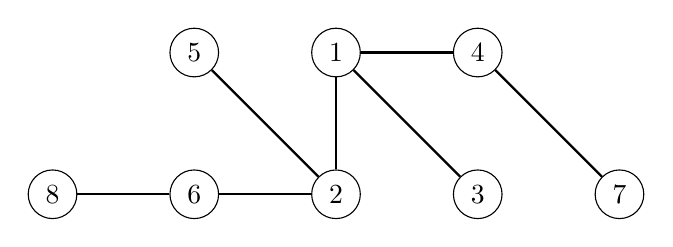
\begin{tikzpicture}[scale=0.9]
\node[draw, circle] (1) at (0,3) {$1$};
\node[draw, circle] (2) at (2,3) {$4$};
\node[draw, circle] (3) at (0,1) {$2$};
\node[draw, circle] (4) at (2,1) {$3$};
\node[draw, circle] (5) at (4,1) {$7$};
\node[draw, circle] (6) at (-2,3) {$5$};
\node[draw, circle] (7) at (-2,1) {$6$};
\node[draw, circle] (8) at (-4,1) {$8$};
\path[draw,thick,-] (1) -- (2);
\path[draw,thick,-] (1) -- (3);
\path[draw,thick,-] (1) -- (4);
\path[draw,thick,-] (2) -- (5);
\path[draw,thick,-] (3) -- (6);
\path[draw,thick,-] (3) -- (7);
\path[draw,thick,-] (7) -- (8);
\end{tikzpicture}
\end{center}

\index{leaf}

As \key{folhas} de uma árvore são os nós com grau 1, ou seja, com apenas um vizinho. Por exemplo, as folhas da árvore acima são os nós 3, 5, 7 e 8.

\index{root}
\index{rooted tree}

Em uma árvore \key{enraizada}, um dos nós é designado como a \key{raiz} da árvore, e todos os outros nós são colocados abaixo da raiz. Por exemplo, na árvore a seguir, o nó 1 é o nó raiz.

\begin{center}
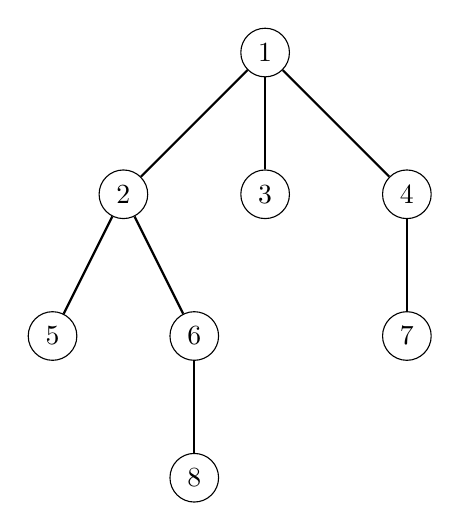
\begin{tikzpicture}[scale=0.9]
\node[draw, circle] (1) at (0,3) {$1$};
\node[draw, circle] (4) at (2,1) {$4$};
\node[draw, circle] (2) at (-2,1) {$2$};
\node[draw, circle] (3) at (0,1) {$3$};
\node[draw, circle] (7) at (2,-1) {$7$};
\node[draw, circle] (5) at (-3,-1) {$5$};
\node[draw, circle] (6) at (-1,-1) {$6$};
\node[draw, circle] (8) at (-1,-3) {$8$};
\path[draw,thick,-] (1) -- (2);
\path[draw,thick,-] (1) -- (3);
\path[draw,thick,-] (1) -- (4);
\path[draw,thick,-] (2) -- (5);
\path[draw,thick,-] (2) -- (6);
\path[draw,thick,-] (4) -- (7);
\path[draw,thick,-] (6) -- (8);
\end{tikzpicture}
\end{center}

\index{child}
\index{parent}

Em uma árvore enraizada, os \key{filhos} de um nó são seus vizinhos inferiores e o \key{pai} de um nó é seu vizinho superior. Cada nó tem exatamente um pai, exceto pela raiz que não possui pai. Por exemplo, na árvore acima, os filhos do nó 2 são os nós 5 e 6, e seu pai é o nó 1.

\index{subtree}

A estrutura de uma árvore enraizada é \emph{recursiva}: cada nó da árvore atua como a raiz de uma \key{subárvore} que contém o próprio nó e todos os nós que estão nas subárvores de seus filhos. Por exemplo, na árvore acima, a subárvore do nó 2 consiste nos nós 2, 5, 6 e 8:
\begin{center}
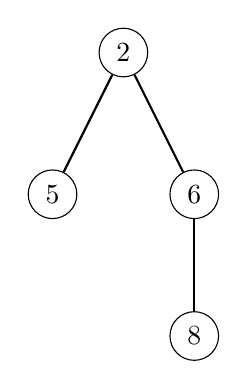
\begin{tikzpicture}[scale=0.9]
\node[draw, circle] (2) at (-2,1) {$2$};
\node[draw, circle] (5) at (-3,-1) {$5$};
\node[draw, circle] (6) at (-1,-1) {$6$};
\node[draw, circle] (8) at (-1,-3) {$8$};
\path[draw,thick,-] (2) -- (5);
\path[draw,thick,-] (2) -- (6);
\path[draw,thick,-] (6) -- (8);
\end{tikzpicture}
\end{center}

\section{Travessia de Árvore}

Algoritmos gerais de travessia de grafos podem ser usados para percorrer os nós de uma árvore. No entanto, a travessia de uma árvore é mais fácil de implementar do que a de um grafo geral, pois não há ciclos na árvore e não é possível alcançar um nó por múltiplas direções.

A maneira típica de percorrer uma árvore é iniciar uma busca em profundidade em um nó arbitrário. A seguinte função recursiva pode ser usada:

\begin{lstlisting}
void dfs(int s, int e) {
    // processa o no s
    for (auto u : adj[s]) {
        if (u != e) dfs(u, s);
    }
}
\end{lstlisting}

A função recebe dois parâmetros: o nó atual $s$ e o nó anterior $e$. O objetivo do parâmetro $e$ é garantir que a busca se mova apenas para nós que ainda não foram visitados.

A seguinte chamada de função inicia a busca no nó $x$:

\begin{lstlisting}
dfs(x, 0);
\end{lstlisting}

Na primeira chamada $e=0$, pois não há nó anterior, e é permitido prosseguir em qualquer direção na árvore.

\subsubsection{Programação Dinâmica}

A programação dinâmica pode ser usada para calcular algumas informações durante a travessia de uma árvore. Usando programação dinâmica, podemos, por exemplo, calcular em tempo $O(n)$ para cada nó de uma árvore enraizada o número de nós em sua subárvore ou o comprimento do caminho mais longo do nó até uma folha.

Como exemplo, vamos calcular para cada nó $s$ um valor $\texttt{count}[s]$: o número de nós em sua subárvore. A subárvore contém o próprio nó e todos os nós nas subárvores de seus filhos, então podemos calcular o número de nós recursivamente usando o seguinte código:

\begin{lstlisting}
void dfs(int s, int e) {
    count[s] = 1;
    for (auto u : adj[s]) {
        if (u == e) continue;
        dfs(u, s);
        count[s] += count[u];
    }
}
\end{lstlisting}

\section{Diâmetro}

\index{diameter}

O \key{diâmetro} de uma árvore é o comprimento máximo de um caminho entre dois nós. Por exemplo, considere a seguinte árvore:
\begin{center}
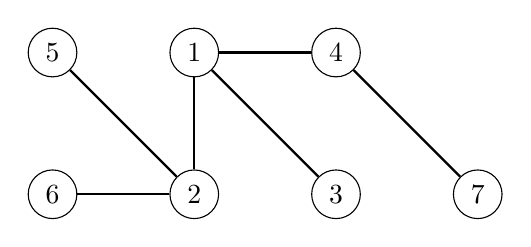
\begin{tikzpicture}[scale=0.9]
\node[draw, circle] (1) at (0,3) {$1$};
\node[draw, circle] (2) at (2,3) {$4$};
\node[draw, circle] (3) at (0,1) {$2$};
\node[draw, circle] (4) at (2,1) {$3$};
\node[draw, circle] (5) at (4,1) {$7$};
\node[draw, circle] (6) at (-2,3) {$5$};
\node[draw, circle] (7) at (-2,1) {$6$};
\path[draw,thick,-] (1) -- (2);
\path[draw,thick,-] (1) -- (3);
\path[draw,thick,-] (1) -- (4);
\path[draw,thick,-] (2) -- (5);
\path[draw,thick,-] (3) -- (6);
\path[draw,thick,-] (3) -- (7);
\end{tikzpicture}
\end{center}
O diâmetro desta árvore é 4, o que corresponde ao seguinte caminho:
\begin{center}
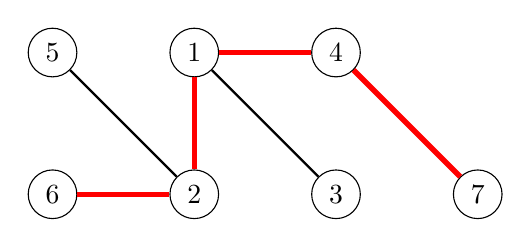
\begin{tikzpicture}[scale=0.9]
\node[draw, circle] (1) at (0,3) {$1$};
\node[draw, circle] (2) at (2,3) {$4$};
\node[draw, circle] (3) at (0,1) {$2$};
\node[draw, circle] (4) at (2,1) {$3$};
\node[draw, circle] (5) at (4,1) {$7$};
\node[draw, circle] (6) at (-2,3) {$5$};
\node[draw, circle] (7) at (-2,1) {$6$};
\path[draw,thick,-] (1) -- (2);
\path[draw,thick,-] (1) -- (3);
\path[draw,thick,-] (1) -- (4);
\path[draw,thick,-] (2) -- (5);
\path[draw,thick,-] (3) -- (6);
\path[draw,thick,-] (3) -- (7);

\path[draw,thick,-,color=red,line width=2pt] (7) -- (3);
\path[draw,thick,-,color=red,line width=2pt] (3) -- (1);
\path[draw,thick,-,color=red,line width=2pt] (1) -- (2);
\path[draw,thick,-,color=red,line width=2pt] (2) -- (5);
\end{tikzpicture}
\end{center}
Observe que pode haver vários caminhos de comprimento máximo. No caminho acima, poderíamos substituir o nó 6 pelo nó 5 para obter outro caminho com comprimento 4.

A seguir, discutiremos dois algoritmos de tempo $O(n)$ para calcular o diâmetro de uma árvore. O primeiro algoritmo é baseado em programação dinâmica e o segundo algoritmo usa duas buscas em profundidade.

\subsubsection{Algoritmo 1}

Uma maneira geral de abordar muitos problemas de árvore é primeiro enraizar a árvore arbitrariamente. Depois disso, podemos tentar resolver o problema separadamente para cada subárvore. Nosso primeiro algoritmo para calcular o diâmetro é baseado nessa ideia.

Uma observação importante é que todo caminho em uma árvore enraizada tem um \emph{ponto mais alto}: o nó mais alto que pertence ao caminho. Assim, podemos calcular para cada nó o comprimento do caminho mais longo cujo ponto mais alto é o nó. Um desses caminhos corresponde ao diâmetro da árvore.

Por exemplo, na árvore a seguir, o nó 1 é o ponto mais alto no caminho que corresponde ao diâmetro:
\begin{center}
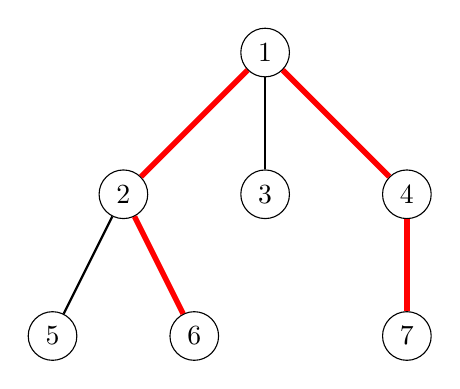
\begin{tikzpicture}[scale=0.9]
\node[draw, circle] (1) at (0,3) {$1$};
\node[draw, circle] (2) at (2,1) {$4$};
\node[draw, circle] (3) at (-2,1) {$2$};
\node[draw, circle] (4) at (0,1) {$3$};
\node[draw, circle] (5) at (2,-1) {$7$};
\node[draw, circle] (6) at (-3,-1) {$5$};
\node[draw, circle] (7) at (-1,-1) {$6$};
\path[draw,thick,-] (1) -- (2);
\path[draw,thick,-] (1) -- (3);
\path[draw,thick,-] (1) -- (4);
\path[draw,thick,-] (2) -- (5);
\path[draw,thick,-] (3) -- (6);
\path[draw,thick,-] (3) -- (7);

\path[draw,thick,-,color=red,line width=2pt] (7) -- (3);
\path[draw,thick,-,color=red,line width=2pt] (3) -- (1);
\path[draw,thick,-,color=red,line width=2pt] (1) -- (2);
\path[draw,thick,-,color=red,line width=2pt] (2) -- (5);
\end{tikzpicture}
\end{center}

Calculamos para cada nó $x$ dois valores:
\begin{itemize}
\item $\texttt{toLeaf}(x)$: o comprimento máximo de um caminho de $x$ até qualquer folha
\item $\texttt{maxLength}(x)$: o comprimento máximo de um caminho cujo ponto mais alto é $x$
\end{itemize}
Por exemplo, na árvore acima, $\texttt{toLeaf}(1)=2$, pois há um caminho $1 \rightarrow 2 \rightarrow 6$, e $\texttt{maxLength}(1)=4$, pois há um caminho $6 \rightarrow 2 \rightarrow 1 \rightarrow 4 \rightarrow 7$. Neste caso, $\texttt{maxLength}(1)$ é igual ao diâmetro.

A programação dinâmica pode ser usada para calcular os valores acima para todos os nós em tempo $O(n)$. Primeiro, para calcular $\texttt{toLeaf}(x)$, percorremos os filhos de $x$, escolhemos um filho $c$ com o máximo $\texttt{toLeaf}(c)$ e adicionamos um a esse valor. Então, para calcular $\texttt{maxLength}(x)$, escolhemos dois filhos distintos $a$ e $b$ tais que a soma $\texttt{toLeaf}(a)+\texttt{toLeaf}(b)$ seja máxima e adicionamos dois a essa soma.

\subsubsection{Algoritmo 2}

Outra maneira eficiente de calcular o diâmetro de uma árvore é baseada em duas buscas em profundidade. Primeiro, escolhemos um nó arbitrário $a$ na árvore e encontramos o nó $b$ mais distante de $a$. Então, encontramos o nó $c$ mais distante de $b$. O diâmetro da árvore é a distância entre $b$ e $c$.

No seguinte gráfico, $a$, $b$ e $c$ podem ser:
\begin{center}
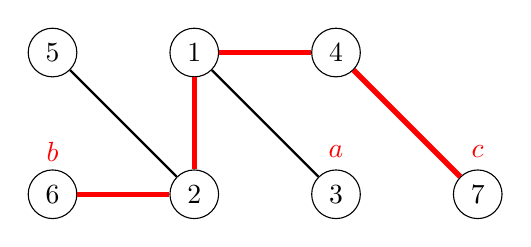
\begin{tikzpicture}[scale=0.9]
\node[draw, circle] (1) at (0,3) {$1$};
\node[draw, circle] (2) at (2,3) {$4$};
\node[draw, circle] (3) at (0,1) {$2$};
\node[draw, circle] (4) at (2,1) {$3$};
\node[draw, circle] (5) at (4,1) {$7$};
\node[draw, circle] (6) at (-2,3) {$5$};
\node[draw, circle] (7) at (-2,1) {$6$};
\path[draw,thick,-] (1) -- (2);
\path[draw,thick,-] (1) -- (3);
\path[draw,thick,-] (1) -- (4);
\path[draw,thick,-] (2) -- (5);
\path[draw,thick,-] (3) -- (6);
\path[draw,thick,-] (3) -- (7);
\node[color=red] at (2,1.6) {$a$};
\node[color=red] at (-2,1.6) {$b$};
\node[color=red] at (4,1.6) {$c$};

\path[draw,thick,-,color=red,line width=2pt] (7) -- (3);
\path[draw,thick,-,color=red,line width=2pt] (3) -- (1);
\path[draw,thick,-,color=red,line width=2pt] (1) -- (2);
\path[draw,thick,-,color=red,line width=2pt] (2) -- (5);
\end{tikzpicture}
\end{center}

Este é um método elegante, mas por que ele funciona?

Ajuda desenhar a árvore de forma diferente para que o caminho que corresponde ao diâmetro seja horizontal e todos os outros nós pendurados nele:
\begin{center}
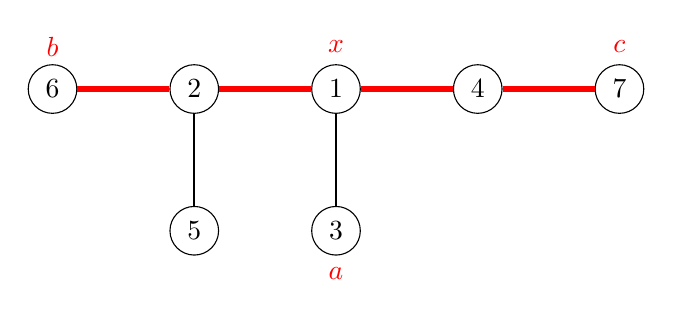
\begin{tikzpicture}[scale=0.9]
\node[draw, circle] (1) at (2,1) {$1$};
\node[draw, circle] (2) at (4,1) {$4$};
\node[draw, circle] (3) at (0,1) {$2$};
\node[draw, circle] (4) at (2,-1) {$3$};
\node[draw, circle] (5) at (6,1) {$7$};
\node[draw, circle] (6) at (0,-1) {$5$};
\node[draw, circle] (7) at (-2,1) {$6$};
\path[draw,thick,-] (1) -- (2);
\path[draw,thick,-] (1) -- (3);
\path[draw,thick,-] (1) -- (4);
\path[draw,thick,-] (2) -- (5);
\path[draw,thick,-] (3) -- (6);
\path[draw,thick,-] (3) -- (7);
\node[color=red] at (2,-1.6) {$a$};
\node[color=red] at (-2,1.6) {$b$};
\node[color=red] at (6,1.6) {$c$};
\node[color=red] at (2,1.6) {$x$};

\path[draw,thick,-,color=red,line width=2pt] (7) -- (3);
\path[draw,thick,-,color=red,line width=2pt] (3) -- (1);
\path[draw,thick,-,color=red,line width=2pt] (1) -- (2);
\path[draw,thick,-,color=red,line width=2pt] (2) -- (5);
\end{tikzpicture}
\end{center}

O nó $x$ indica o local onde o caminho do nó $a$ se junta ao caminho que corresponde ao diâmetro. O nó mais distante de $a$ é o nó $b$, o nó $c$ ou algum outro nó que esteja pelo menos tão distante do nó $x$. Assim, este nó é sempre uma escolha válida para um ponto final de um caminho que corresponde ao diâmetro.

\section{Todos os Caminhos Mais Longos}

Nosso próximo problema é calcular para cada nó na árvore o comprimento máximo de um caminho que começa naquele nó. Isso pode ser visto como uma generalização do problema do diâmetro da árvore, porque o maior desses comprimentos é igual ao diâmetro da árvore. Este problema também pode ser resolvido em tempo $O(n)$.

Como exemplo, considere a seguinte árvore:
\begin{center}
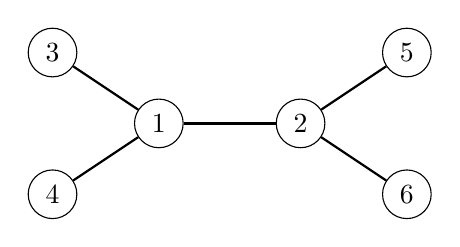
\begin{tikzpicture}[scale=0.9]
\node[draw, circle] (1) at (0,0) {$1$};
\node[draw, circle] (2) at (-1.5,-1) {$4$};
\node[draw, circle] (3) at (2,0) {$2$};
\node[draw, circle] (4) at (-1.5,1) {$3$};
\node[draw, circle] (6) at (3.5,-1) {$6$};
\node[draw, circle] (7) at (3.5,1) {$5$};
\path[draw,thick,-] (1) -- (2);
\path[draw,thick,-] (1) -- (3);
\path[draw,thick,-] (1) -- (4);
\path[draw,thick,-] (3) -- (6);
\path[draw,thick,-] (3) -- (7);
\end{tikzpicture}
\end{center}

Seja $\texttt{maxLength}(x)$ o comprimento máximo de um caminho que começa no nó $x$. Por exemplo, na árvore acima, $\texttt{maxLength}(4)=3$, porque há um caminho $4 \rightarrow 1 \rightarrow 2 \rightarrow 6$. Aqui está uma tabela completa dos valores:
\begin{center}
\begin{tabular}{l|lllllll}
nó $x$ & 1 & 2 & 3 & 4 & 5 & 6 \\
$\texttt{maxLength}(x)$ & 2 & 2 & 3 & 3 & 3 & 3 \\
\end{tabular}
\end{center}

Também neste problema, um bom ponto de partida para resolvê-lo é enraizar a árvore arbitrariamente:
\begin{center}
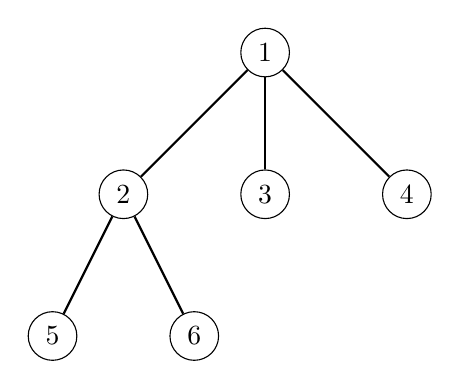
\begin{tikzpicture}[scale=0.9]
\node[draw, circle] (1) at (0,3) {$1$};
\node[draw, circle] (2) at (2,1) {$4$};
\node[draw, circle] (3) at (-2,1) {$2$};
\node[draw, circle] (4) at (0,1) {$3$};
\node[draw, circle] (6) at (-3,-1) {$5$};
\node[draw, circle] (7) at (-1,-1) {$6$};
\path[draw,thick,-] (1) -- (2);
\path[draw,thick,-] (1) -- (3);
\path[draw,thick,-] (1) -- (4);
\path[draw,thick,-] (3) -- (6);
\path[draw,thick,-] (3) -- (7);
\end{tikzpicture}
\end{center}

A primeira parte do problema é calcular para cada nó $x$ o comprimento máximo de um caminho que passa por um filho de $x$. Por exemplo, o caminho mais longo do nó 1 passa por seu filho 2:
\begin{center}
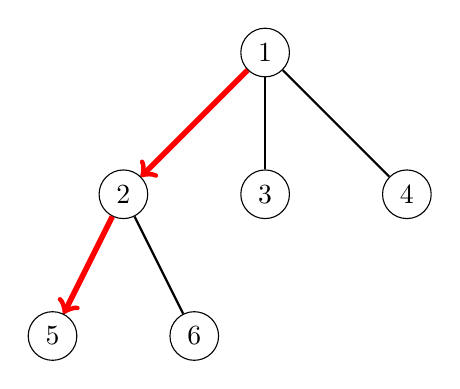
\begin{tikzpicture}[scale=0.9]
\node[draw, circle] (1) at (0,3) {$1$};
\node[draw, circle] (2) at (2,1) {$4$};
\node[draw, circle] (3) at (-2,1) {$2$};
\node[draw, circle] (4) at (0,1) {$3$};
\node[draw, circle] (6) at (-3,-1) {$5$};
\node[draw, circle] (7) at (-1,-1) {$6$};
\path[draw,thick,-] (1) -- (2);
\path[draw,thick,-] (1) -- (3);
\path[draw,thick,-] (1) -- (4);
\path[draw,thick,-] (3) -- (6);
\path[draw,thick,-] (3) -- (7);

\path[draw,thick,->,color=red,line width=2pt] (1) -- (3);
\path[draw,thick,->,color=red,line width=2pt] (3) -- (6);
\end{tikzpicture}
\end{center}
Esta parte é fácil de resolver em tempo $O(n)$, pois podemos usar a programação dinâmica como fizemos anteriormente.

Então, a segunda parte do problema é calcular para cada nó $x$ o comprimento máximo de um caminho através de seu pai $p$. Por exemplo, o caminho mais longo do nó 3 passa por seu pai 1:
\begin{center}
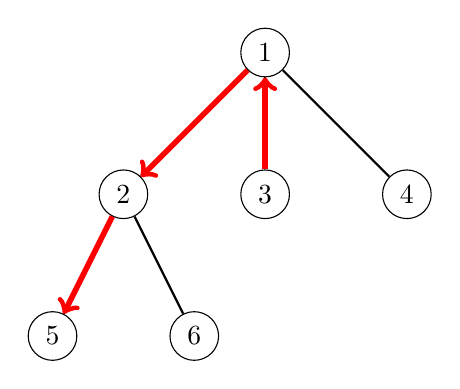
\begin{tikzpicture}[scale=0.9]
\node[draw, circle] (1) at (0,3) {$1$};
\node[draw, circle] (2) at (2,1) {$4$};
\node[draw, circle] (3) at (-2,1) {$2$};
\node[draw, circle] (4) at (0,1) {$3$};
\node[draw, circle] (6) at (-3,-1) {$5$};
\node[draw, circle] (7) at (-1,-1) {$6$};
\path[draw,thick,-] (1) -- (2);
\path[draw,thick,-] (1) -- (3);
\path[draw,thick,-] (1) -- (4);
\path[draw,thick,-] (3) -- (6);
\path[draw,thick,-] (3) -- (7);

\path[draw,thick,->,color=red,line width=2pt] (4) -- (1);
\path[draw,thick,->,color=red,line width=2pt] (1) -- (3);
\path[draw,thick,->,color=red,line width=2pt] (3) -- (6);
\end{tikzpicture}
\end{center}

À primeira vista, parece que devemos escolher o caminho mais longo de $p$. No entanto, isso \emph{não} funciona sempre, porque o caminho mais longo de $p$ pode passar por $x$. Aqui está um exemplo desta situação:
\begin{center}
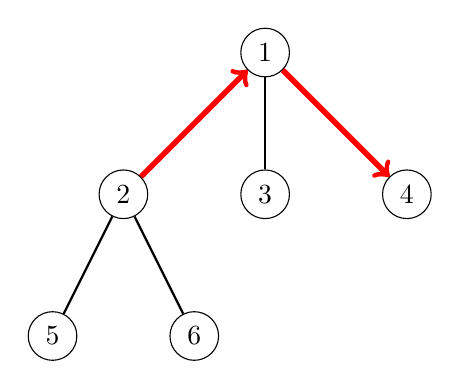
\begin{tikzpicture}[scale=0.9]
\node[draw, circle] (1) at (0,3) {$1$};
\node[draw, circle] (2) at (2,1) {$4$};
\node[draw, circle] (3) at (-2,1) {$2$};
\node[draw, circle] (4) at (0,1) {$3$};
\node[draw, circle] (6) at (-3,-1) {$5$};
\node[draw, circle] (7) at (-1,-1) {$6$};
\path[draw,thick,-] (1) -- (2);
\path[draw,thick,-] (1) -- (3);
\path[draw,thick,-] (1) -- (4);
\path[draw,thick,-] (3) -- (6);
\path[draw,thick,-] (3) -- (7);

\path[draw,thick,->,color=red,line width=2pt] (3) -- (1);
\path[draw,thick,->,color=red,line width=2pt] (1) -- (2);
\end{tikzpicture}
\end{center}

Ainda assim, podemos resolver a segunda parte em tempo $O(n)$ armazenando \emph{dois} comprimentos máximos para cada nó $x$:
\begin{itemize}
\item $\texttt{maxLength}_1(x)$: o comprimento máximo de um caminho de $x$
\item $\texttt{maxLength}_2(x)$: o comprimento máximo de um caminho de $x$ em outra direção que não o primeiro caminho
\end{itemize}
Por exemplo, no gráfico acima, $\texttt{maxLength}_1(1)=2$ usando o caminho $1 \rightarrow 2 \rightarrow 5$ e $\texttt{maxLength}_2(1)=1$ usando o caminho $1 \rightarrow 3$.

Finalmente, se o caminho que corresponde a $\texttt{maxLength}_1(p)$ passa por $x$, concluímos que o comprimento máximo é $\texttt{maxLength}_2(p)+1$, caso contrário, o comprimento máximo é $\texttt{maxLength}_1(p)+1$.

\section{Árvores Binárias}

\index{binary tree}

\begin{samepage}
Uma \key{árvore binária} é uma árvore enraizada onde cada nó possui uma subárvore esquerda e uma subárvore direita. É possível que uma subárvore de um nó esteja vazia. Assim, todo nó em uma árvore binária tem zero, um ou dois filhos.

Por exemplo, a seguinte árvore é uma árvore binária:
\begin{center}
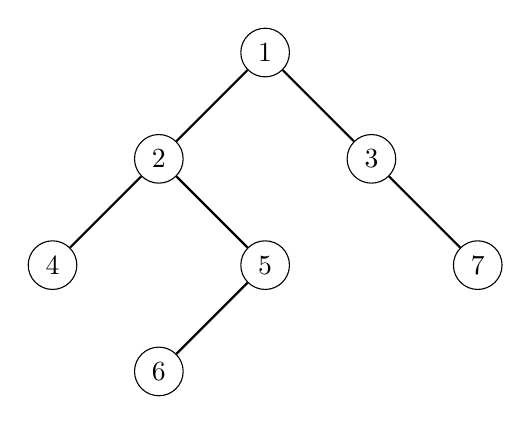
\begin{tikzpicture}[scale=0.9]
\node[draw, circle] (1) at (0,0) {$1$};
\node[draw, circle] (2) at (-1.5,-1.5) {$2$};
\node[draw, circle] (3) at (1.5,-1.5) {$3$};
\node[draw, circle] (4) at (-3,-3) {$4$};
\node[draw, circle] (5) at (0,-3) {$5$};
\node[draw, circle] (6) at (-1.5,-4.5) {$6$};
\node[draw, circle] (7) at (3,-3) {$7$};

\path[draw,thick,-] (1) -- (2);
\path[draw,thick,-] (1) -- (3);
\path[draw,thick,-] (2) -- (4);
\path[draw,thick,-] (2) -- (5);
\path[draw,thick,-] (5) -- (6);
\path[draw,thick,-] (3) -- (7);
\end{tikzpicture}
\end{center}
\end{samepage}

\index{pre-order}
\index{in-order}
\index{post-order}

Os nós de uma árvore binária possuem três ordenações naturais que correspondem a diferentes maneiras de percorrer recursivamente a árvore:

\begin{itemize}
\item \key{pré-ordem}: primeiro processa a raiz, depois percorre a subárvore esquerda e, em seguida, percorre a subárvore direita
\item \key{em-ordem}: primeiro percorre a subárvore esquerda, depois processa a raiz e, em seguida, percorre a subárvore direita
\item \key{pós-ordem}: primeiro percorre a subárvore esquerda, depois percorre a subárvore direita e, em seguida, processa a raiz
\end{itemize}

Para a árvore acima, os nós em pré-ordem são $[1,2,4,5,6,3,7]$, em ordem $[4,2,6,5,1,3,7]$ e em pós-ordem $[4,6,5,2,7,3,1]$.

Se conhecermos a pré-ordem e a ordem de uma árvore, podemos reconstruir a estrutura exata da árvore. Por exemplo, a árvore acima é a única árvore possível com pré-ordem $[1,2,4,5,6,3,7]$ e ordem $[4,2,6,5,1,3,7]$. De forma semelhante, a pós-ordem e a ordem também determinam a estrutura de uma árvore.

No entanto, a situação é diferente se conhecermos apenas a pré-ordem e a pós-ordem de uma árvore. Nesse caso, pode haver mais de uma árvore que corresponda às ordenações. Por exemplo, em ambas as árvores
\begin{center}
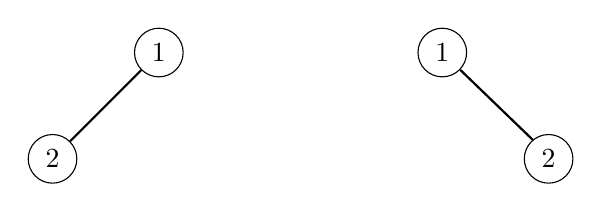
\begin{tikzpicture}[scale=0.9]
\node[draw, circle] (1) at (0,0) {$1$};
\node[draw, circle] (2) at (-1.5,-1.5) {$2$};
\path[draw,thick,-] (1) -- (2);

\node[draw, circle] (1b) at (0+4,0) {$1$};
\node[draw, circle] (2b) at (1.5+4,-1.5) {$2$};
\path[draw,thick,-] (1b) -- (2b);
\end{tikzpicture}
\end{center}
a pré-ordem é $[1,2]$ e a pós-ordem é $[2,1]$, mas as estruturas das árvores são diferentes.
